The data-driven methods described so far use the forecast of features to obtain building power consumption predictions  for DR baseline and DR strategy evaluation.
In this section, we extend the theory of regression trees to solve the demand response synthesis problem described earlier in Sec.~\ref{sec:synthesis}. This is one of our primary contribution.

\begin{figure}
\centering
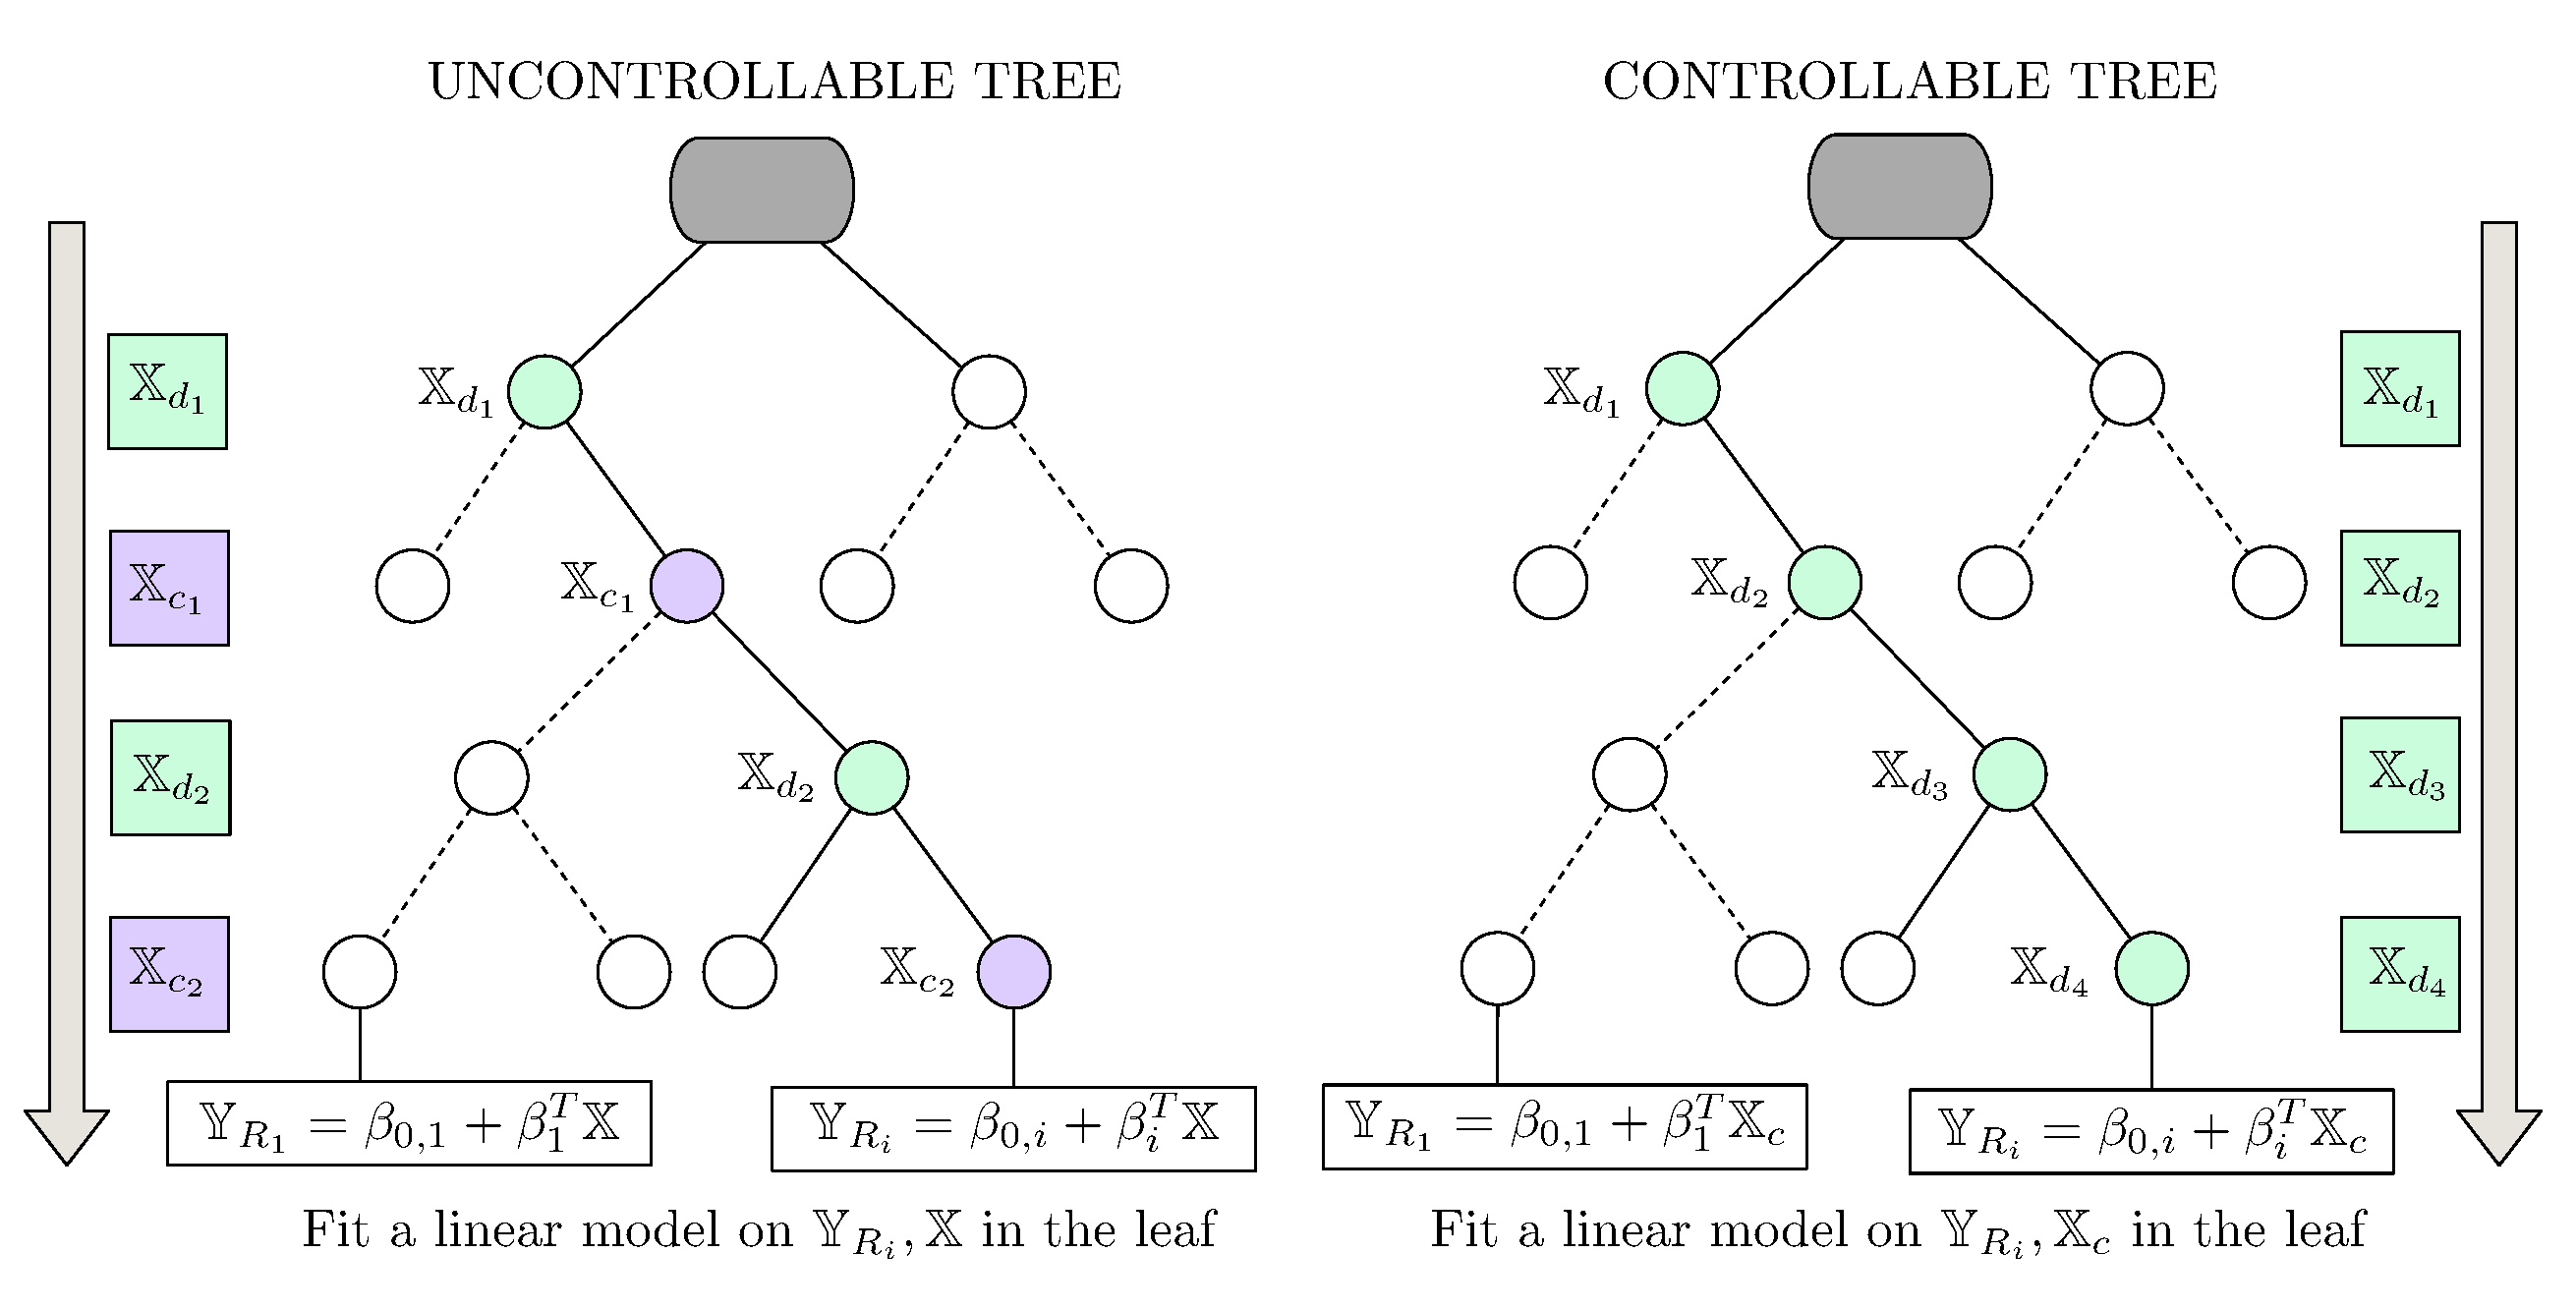
\includegraphics[width=0.95\columnwidth]{Figures/sep_vars.eps}
   \caption{Left: Example of a regression tree not suitable for control due to the mixed order of the controllable $\mathbb{X}_c$ and uncontrollable $\mathbb{X}_d$ features. Right: Example of a tree structure obtained used for mbCRT algorithm. The separation of variables allows using the linear model in the leaf to use only control variables.}
   \captionsetup{justification=centering}
   \label{fig:training}
\end{figure}
%\begin{figure*}
%\centering
%\begin{subfigure}
%  \centering
%  \includegraphics[width=0.4\columnwidth]{figs/mixed_order}
%  \end{subfigure}  
%  \begin{subfigure}
%    \centering
%  \includegraphics[width=0.5\columnwidth]{figs/sepofv-compressed}
%  \end{subfigure}
%   \caption{Left: Example of a regression tree not suitable for control due to the mixed order of the controllable $X_c$ (solid blue) and uncontrollable $X_d$ features. Right: Example of a tree structure obtained used for mbCRT algorithm. The separation of variables allows using the linear model in the leaf to use only control variables.}
%   \captionsetup{justification=centering}
%   \label{fig:training}
%\end{figure*}

Recall that the objective of learning a regression tree is to learn a model $f$ for predicting the response $\mathbb{Y}$ with the values of the predictor variables or features $\mathbb{X}^1, \dots, \mathbb{X}^n$; i.e. $\mathbb{Y}=f(\mathbb{X}^1, \dots, \mathbb{X}^n)$.
Given a forecast of the features $\hat{X}^1, \dots, \hat{X}^n$, we can predict the response $\hat{Y}$. 
Now consider the case where a subset, $\mathbb{X}_c \subset \mathbb{X}$ of the set of features/variables $\mathbb{X}$'s are manipulated variables i.e. we can change their values in order to drive the response $\mathbb{Y}$ towards a certain value. 
In the case of buildings, the set of  variables can be separated into disturbances (or non-manipulated) variables like outside air temperature, humidity, wind etc. while the controllable (or manipulated) variables would be the temperature and lighting set-points within the building.
Our goal is to modify the regression trees and make them suitable for synthesizing the optimal values of the control variables in real-time.

\subsection{Model-based control with regression trees}
\label{sec:mbcrt}

The key idea in enabling control synthesis for regression trees is in the separation of features/variables into manipulated and non-manipulated features. 
Let $\mathbb{X}_c \subset \mathbb{X}$ denote the set of manipulated variables and $\mathbb{X}_d \subset \mathbb{X}$ denote the set of disturbances/ non-manipulated variables such that $\mathbb{X}_c \cup \mathbb{X}_d \equiv \mathbb{X}$.
Using this separation of variables, we build upon the idea of simple model based regression trees~\cite{friedman1991multivariate} to \emph{model based control with regression trees (mbCRT)}. 

Fig.~\ref{fig:training} (L) shows an example of how manipulated and non-manipulated features can get distributed at different depths of model based regression tree which uses the a linear regression function in the leaves of the tree:
%\begin{equation}
%\hat{Y_{Ri}} = \beta_{0,i} + \beta^T_i \mathbb{X}
%\end{equation}
\begin{gather}
\mathbb{Y}_{R_i} = \beta_{0,i} + \beta^T_i \mathbb{X},
\label{eq:linear_regression_leaf}
\end{gather}
where $\mathbb{Y}_{R_i}$ is the predicted response in region $R_i$ of the tree using all the features $\mathbb{X}$. 
 In such a tree the prediction can only be obtained if the values of all the features $\mathbb{X}$ are known, including the values of the control variables $\mathbb{X}_c$. 
Since the manipulated and non-manipulated variables appear in a mixed order in the tree depth, we cannot use this tree for control synthesis.
This is because the values of the control variables $\mathbb{X}_{c}$ are unknown, one cannot navigate to any single region using the forecast of disturbances alone. 
%\begin{figure}
%  \centering
%  \includegraphics[width=0.8\columnwidth]{figs/sepofv-compressed}
%  \caption{Example of a tree structure obtained using the mbCRT algorithm. The separation of variables allows using the linear model in the leaf to use only control variables.}
%  \label{fig:algo1}
%\end{figure}

The mbCRT algorithm avoids this problem using a simple but clever idea. We still partition the entire data space into regions using CART algorithm, but the top part of the regression tree is learned only on the non-manipulated features $\mathbb{X}_d$ or disturbances as opposed to all the features $\mathbb{X}$ as shown in Fig.~\ref{fig:training} (R).
In every region at the leaves of the ``disturbance'' tree a linear model is fit but only on the control variables $\mathbb{X}_c$:
\begin{equation}
\mathbb{Y}_{R_i} = \beta_{0,i} + \beta^T_i \mathbb{X}_c.
\label{eq:control_leaf}
\end{equation}
Separation of variables allows us to use the forecast of the disturbances $\mathbb{X}_d$ to navigate to the appropriate region $R_i$ and use the linear regression model $\mathbb{Y}_{R_i} = \beta_{0,i} + \beta^T_i \mathbb{X}_c$ with only the control/manipulated features in it as the valid prediction model for that time-step.

\begin{algorithm}[t]
\caption{mbCRT: Model Based Control With Regression Trees}\label{alg:mbcrt}
\begin{algorithmic}[]
\State \textsc{Design Time}
\Procedure{Model Training using Separation of Variables}{}
\State Set $\mathbb{X}_c$ $\gets$ manipulated features
\State Set $\mathbb{X}_d$ $\gets$ non-manipulated features
\State Build the power prediction tree $\mathcal{P}$ with $\mathbb{X}_d$
\ForAll{Regions $R_i$ at the leaves of $\mathcal{P}$}
\State Fit a linear model $\mathcal{P}_{R_i} = \beta_{0,i} + \beta^T_i \mathbb{X}_c$
\EndFor
\State Build $q$ temperature trees $\mathcal{T}^1,\mathcal{T}^2, \dots, \mathcal{T}^q$ with $\mathbb{X}_d$
\ForAll{Regions $R_i$ at the leaves of $\mathcal{T}^j$}
\State Fit a linear model $\mathcal{T}_{R_i}^j = \alpha_{0,i}^j + {\alpha^j}^T_i \mathbb{X}_c$
\EndFor
\EndProcedure
\State \textsc{Run Time}
\Procedure{Control Synthesis}{}
\While{$t< t_{\mathrm{stop}}$}
\State Determine forecast $\mathbb{X}_d(t)$ of disturbances
\State Determine the leaf and regions $R_{i}(t)$ for each tree using $\mathbb{X}_d(t)$
\State Obtain the linear model at the leaf of each tree
\State Solve optimization in \eqref{eq:synth_program} to determine optimal control action $\mathbb{X}^*_c(t)$
\EndWhile
\EndProcedure
\end{algorithmic}
\end{algorithm}

\begin{figure}[h]
\centering
%\includegraphics[width=0.5\columnwidth]{figs/alg1new}
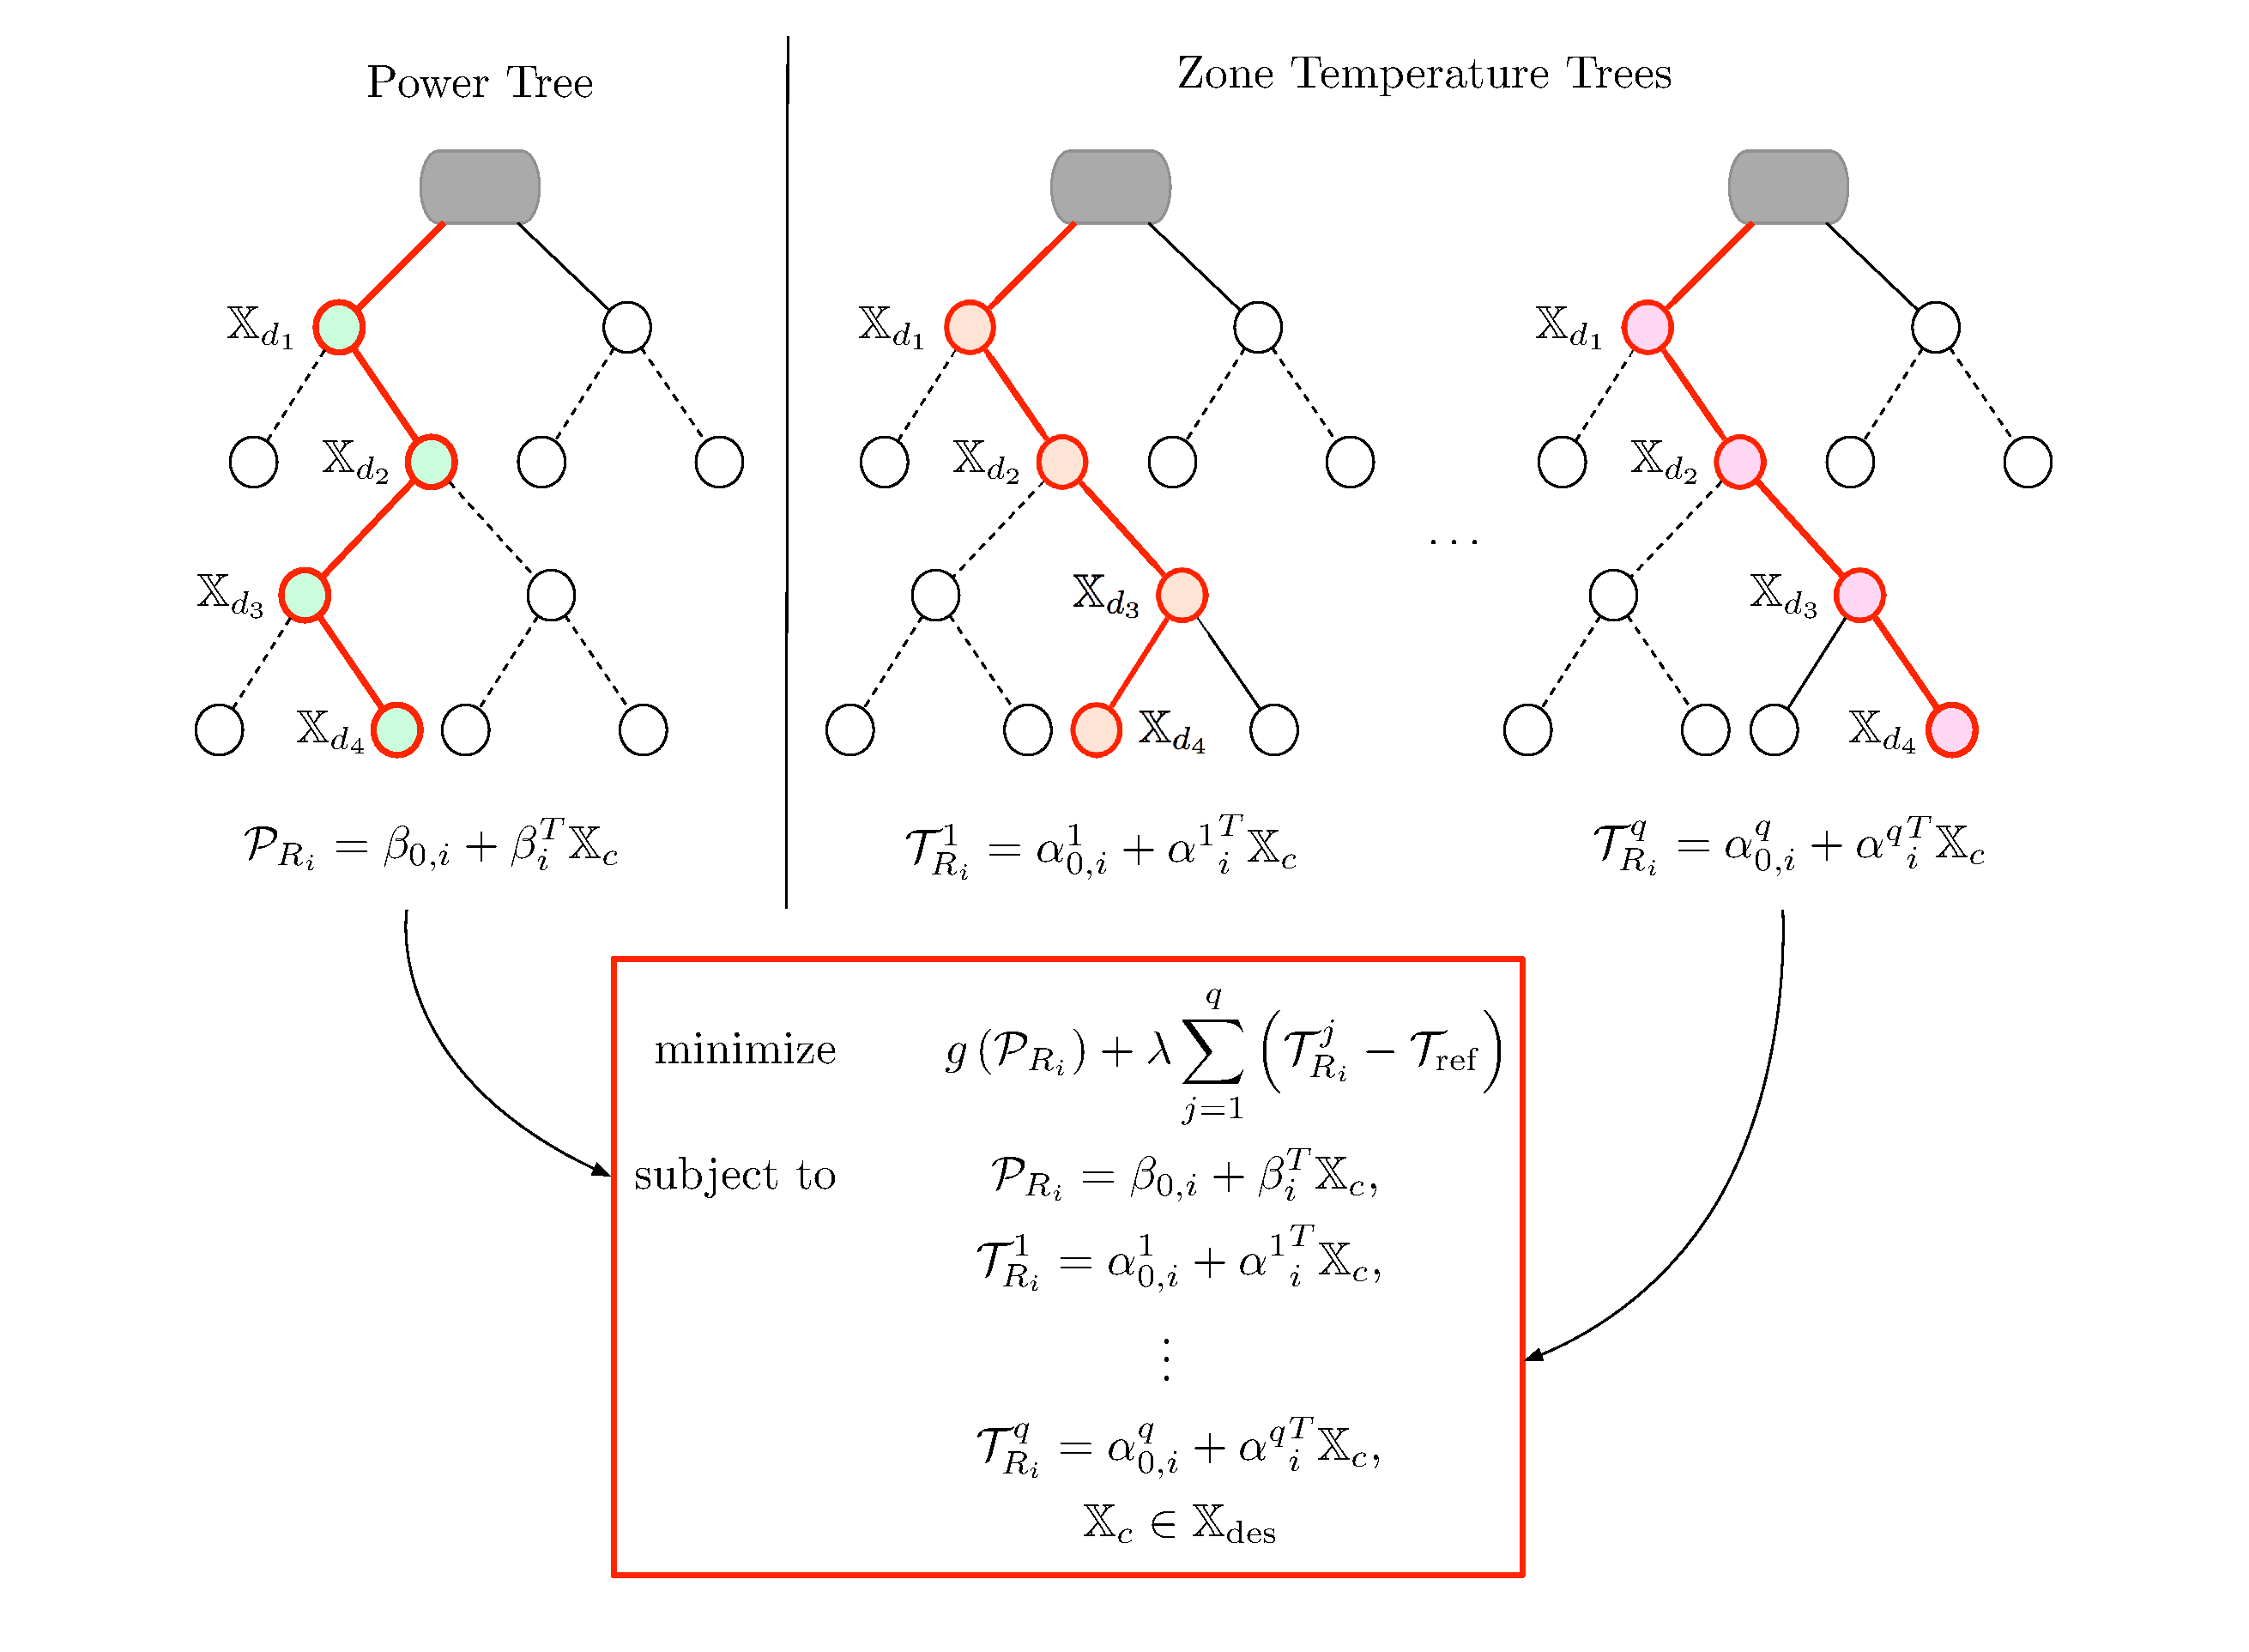
\includegraphics[width=0.95\columnwidth]{Figures/mbCRT.eps}
\caption{DR synthesis with thermal comfort constraints. Each tree is responsible for contributing one constraint to the demand response optimization.}
\label{fig:dropt}
\end{figure}

\subsection{DR synthesis optimization}
In the case of DR synthesis for buildings, the response variable is power consumption, and the objective function can denote the financial reward of minimizing the power consumption during the DR event. However, the curtailment must not result in high levels of discomfort for the building occupants. In order to account for thermal comfort, in addition to learning the tree for power consumption forecast, we can also learn different trees to predict the temperature of different zones in the building. As shown in Fig.~\ref{fig:dropt} and Algo.~\ref{alg:mbcrt}, at each time-step during the DR event, a forecast of the non manipulated variables is used by each tree, to navigate to the appropriate leaf node. For the power forecast tree, the linear model at the leaf node relates the predicted power consumption of the building to the manipulated/control variables, i.e. $\mathcal{P}_{R_i} = \beta_{0,i} + \beta^T_i \mathbb{X}_c$. Similarly, for the $j^{\mathrm{th}}$ zone, a tree is built whose response variable is the zone temperature $\mathcal{T}^j$. The linear model at the leaf node of each of the zone temperature tree relates the predicted zone temperature to the manipulated variables, i.e. $\mathcal{T}_{R_i}^j = \alpha_{0,i}^j + {\alpha^j}^T_i \mathbb{X}_c$.

Therefore, at every time-step, based on the forecast of the non-manipulated variables, we obtain $q+1$ linear models between the power consumption and $q$ zone temperatures and the manipulated variables. We can then solve the following DR synthesis optimization problem to obtain the values of the manipulated variables $\mathbb{X}_c$:

\begin{align}
\begin{aligned}
\text{minimize } \ \ \ & \ \ \ g\left(\mathcal{P}_{R_i}\right) + \lambda \sum_{j=1}^{q} \left( \mathcal{T}^j_{R_i} - \mathcal{T}_{\mathrm{ref}}\right) \\ \text{subject to } \ \ \ &  \ \ \ \ \ \ \mathcal{P}_{R_i} = \beta_{0,i} + \beta^T_i \mathbb{X}_c, \\ \ \ \ & \ \ \ \ \ \mathcal{T}_{R_i}^1 = \alpha_{0,i}^1 + {\alpha^1}^T_i \mathbb{X}_c,  \\ \ \ \ & \ \ \ \ \ \ \ \ \ \ \ \ \ \ \ \ \ \vdots \\ \ \ \ & \ \ \ \ \ \mathcal{T}_{R_i}^q = \alpha_{0,i}^q + {\alpha^q}^T_i \mathbb{X}_c, \\ \ \ \ & \ \ \ \ \ \ \ \ \ \ \ \ \mathbb{X}_c \in \mathbb{X}_{\mathrm{des}}.
  \end{aligned}
\label{eq:synth_program}  
\end{align}
%\begin{center}
%\begin{equation}
%\begin{aligned}
%\underset{\mathbb{X}_c}{\text{minimize}}
% & f(\hat{kW})+\text{Penalty}[\sum_{k=1}^q(\hat{T_k}-T_{ref})] \\
%\text{subject to} \\
%& \hat{kW} = \beta_{0,i} + \beta^T_i \mathbb{X}_c \\
%& \hat{T1} = \alpha_{0,1} + \beta^T_1 \mathbb{X}_c \\
%& \cdots \\
%& \hat{Td} = \alpha_{0,q} + \beta^T_q \mathbb{X}_c \\
%& \mathbb{X}_c \in \mathbb{X}_{safe}
%\end{aligned}
%\label{eq:synth_program}
%\end{equation}
%\end{center}
\begin{figure*}
\centering
  \begin{subfigure}
    \centering
  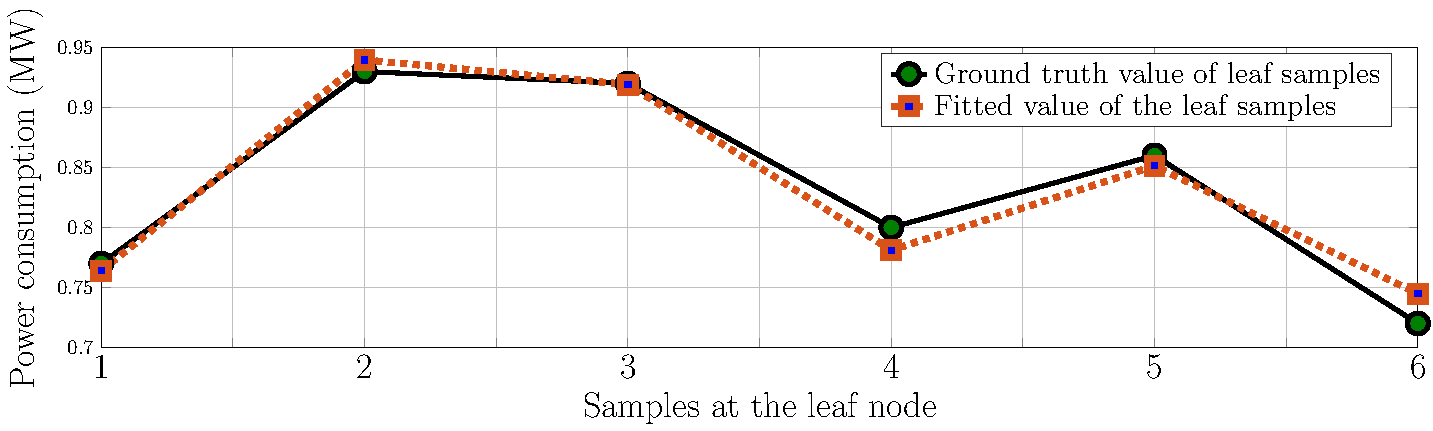
\includegraphics[width=0.7\columnwidth]{figs/leaf200}
  \end{subfigure}  
  \begin{subfigure}
    \centering
  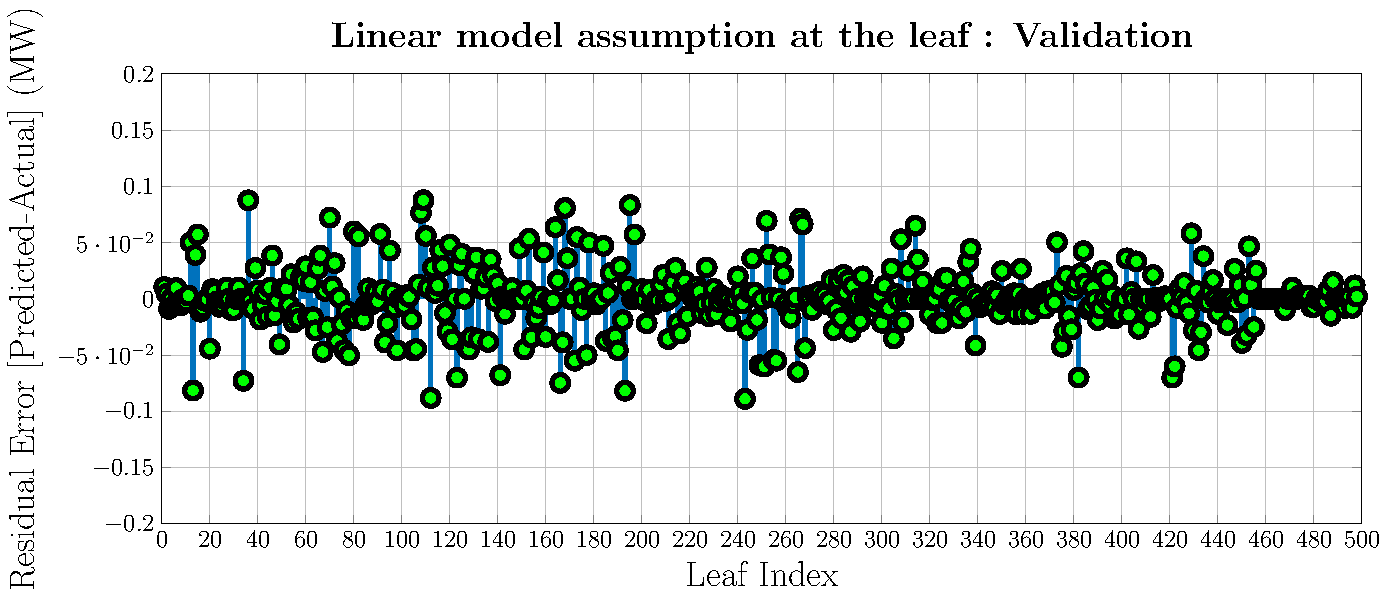
\includegraphics[width=0.7\columnwidth]{figs/goodleaf}
  \end{subfigure}
%   \subfloat{ \centering 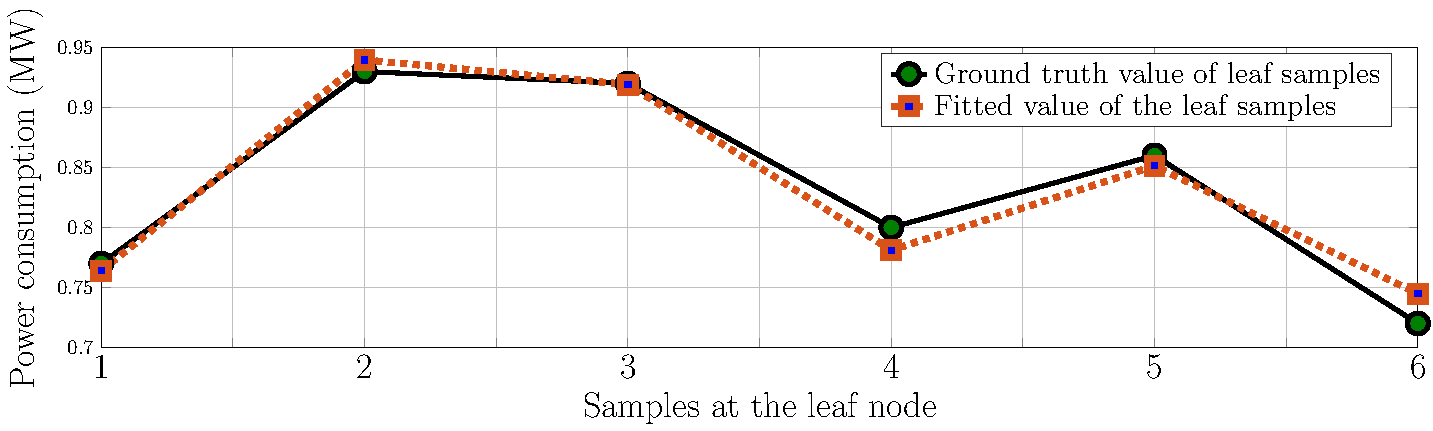
\includegraphics[width=\columnwidth]{figs/leaf200}}  
%  \vfil
%  \centering
%   \subfloat{\centering 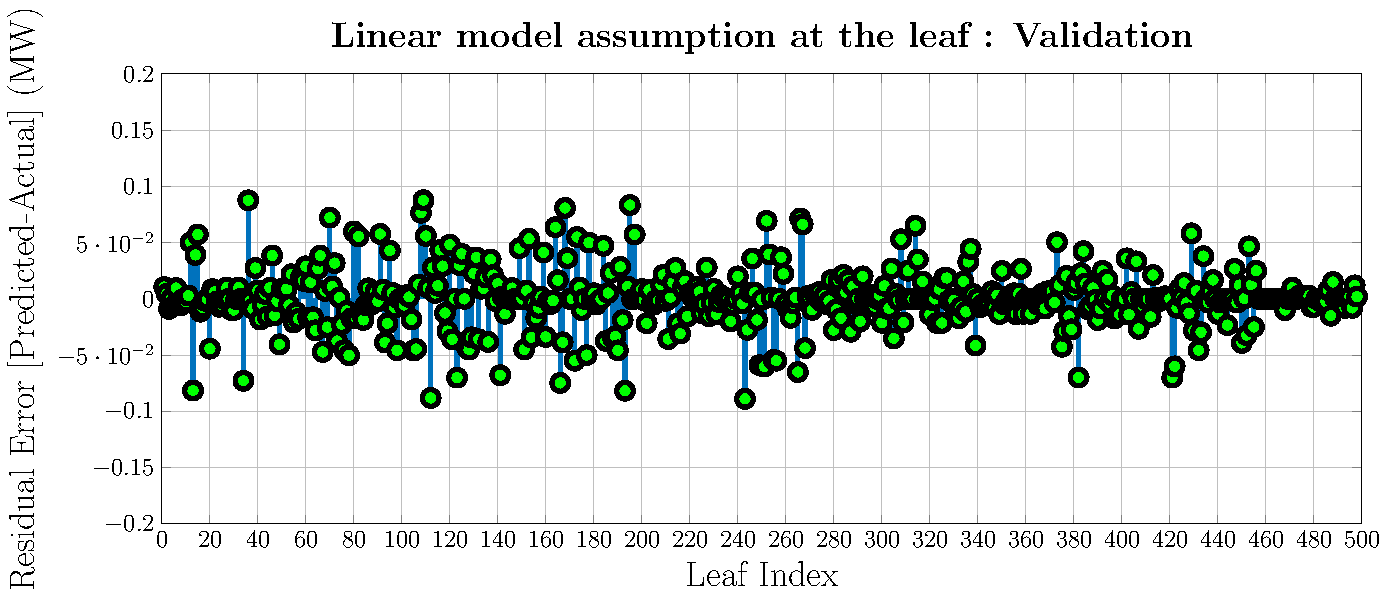
\includegraphics[width=\columnwidth]{figs/goodleaf}}
  \caption{Linear model assumption at the leaves}
  \label{fig:leaf}
\end{figure*}
Here, $\lambda$ is the penalty on the thermal comfort. The linear model between the response variable $\mathcal{P}_{R_i}$ and the control features $\mathbb{X}_c$ is assumed for computational simplicity. Other models could also be used at the leaves as long as they adhere to the separation of variables principle. Fig.~\ref{fig:leaf} shows that the linear model assumption in the leaves of the tree is a valid assumption.

The intuition behind the mbCRT Algo.~\ref{alg:mbcrt} is that at run time $t$, we use the forecast $\mathbb{X}_d(t+1)$ of the disturbance features to determine the leaves of the \textit{controllable} tree and hence, the linear model to be used for the control.
We then solve the simple linear program corresponding to that region to obtain the optimal values of the control variables. 
The mbCRT algorithm is the first ever algorithm which allows the use of regression trees for control synthesis. 
